%%!TEX TS-program = latex
\documentclass[12pt,letterpaper]{article}
\bibliographystyle{evolution}
\usepackage{epsfig}                 
\usepackage[authoryear]{natbib}
\usepackage{graphicx}
\usepackage{amsmath}
\usepackage{psfrag}
\usepackage{mathabx}
\renewcommand{\baselinestretch}{1.6}
\large
\pagenumbering{arabic}
\usepackage[usenames,dvipsnames]{color}
\usepackage{fullpage}
\usepackage{multirow}
\newcommand{\ye}{\hat{y}}
\newcommand{\xe}{\hat{x}}
\usepackage{color}
\usepackage[normalem]{ulem}  
	\newcommand{\gc}[1]{{ \color{red} #1}}
	\newcommand{\yb}[1]{{ \color{blue} #1}}
\usepackage{lineno}
\linenumbers



\title{  Sperm should evolve to make female meiosis fair.  }

\author{Yaniv Brandvain$^1$ \and Graham Coop$^2$ }

\usepackage{fancyhdr}
\pagestyle{fancy}
\lhead{}
\rhead{}
\renewcommand{\headrulewidth}{0.0pt}
\rfoot{}
\cfoot{\thepage}
\date{}
\begin{document}
\maketitle
\begin{center}
$^1$Department of Plant Biology, \\ University of Minnesota -- Twin
Cities. St. Paul MN, 55108 \\
$^2$Center for Population Biology \& Department of Evolution and Ecology \\ University of California -- Davis. Davis, CA, 95616
\end{center}



\newpage

{\bf Abstract:}
Genomic conflicts arise when an allele gains an evolutionary advantage at a cost to organismal fitness. 
O\"{o}genesis is inherently susceptible to such conflicts
because alleles compete for inclusion into the egg. 
Alleles that distort meiosis in their favor (i.e. meiotic drivers) often decrease organismal fitness,
	and therefore indirectly favor the evolution of mechanisms to suppress meiotic drive. 
In this light, many facets of  o\"{o}genesis and gametogenesis have been 
	interpreted as mechanisms of protection against genomic outlaws. 
That females  of many animal species do not complete meiosis until after fertilization, 
     appears to run counter to this interpretation,
     because this delay provides an opportunity for sperm-acting alleles to
     meddle with the outcome of female meiosis and help like alleles drive in heterozygous females. 
Contrary to this perceived danger, the population genetic theory presented herein suggests that, 
	in fact, sperm nearly always evolve to increase the fairness of female
        meiosis in the face of genomic conflicts. 
These results are consistent with the apparent sperm dependence of the best characterized female meiotic drivers in animals.   
Rather than providing an opportunity for sperm collaboration in female meiotic drive,
        the `fertilization requirement'  indirectly protects females from
        meiotic drivers by providing sperm an opportunity to
        suppress drive. 
\newpage

\section*{Introduction}
Despite the apparent unity of the organism, `selfish' alleles can
gain an evolutionary advantage at a cost to  individual fitness
\citep{Burt2006}, often by exploiting meiosis and gametogenesis.
Because only one of the four products of female meiosis is transmitted to the egg, female meiosis is particularly vulnerable to such exploitation \citep{Sandler1957,Pardo-ManuelDeVillena2001a}. 
An allele that biases female meiosis in its favor (i.e. a meiotic driver), can increase in frequency even if it entails a pleiotropic fitness cost \citep{Prout1973}, generating a genetic conflict between the success of the driver and the organism.
Meiotic drivers observed in both plants
\citep{Buckler1999,Fishman2005,Fishman2008}, and animals
\citep{Agulnik1990,Wu2005,Pardo-ManuelDeVillena2001c} highlight this
conflict -- the selfish benefits and the associated
pleiotropic fitness costs of drive sustain a balanced polymorphism
\citep{Prout1973}, 
and often generate ongoing evolutionary escalations of drive suppressors and enhancers \citep{Dawe1996,Fishman2008}. 
The threat of meiotic drive to organismal fitness is potentially so
severe that many basic properties of
meiosis and o\"{o}genesis, including the initial genome doubling in
meiosis I \citep{Haig1991}, arrested female meiosis
\citep{Mira1998}, the structure of centromere machinery \citep{Malik2002a,Malik2009}, and sex differences in the recombination rate \citep{Haig2010,Brandvain2012} 
have perhaps evolved to enforce fairness by disrupting meiotic drive \citep{Rice2013}. \newline 

It is therefore somewhat surprising that despite the intense evolutionary pressure on female meiosis to prevent meiotic drive, 
it is potentially open to sabotage by a virtual stranger -- a haploid sperm genome.
That is, in many animal species, female meiosis is completed only
after fertilization \citep{Masui_book}, creating ample opportunity for interaction between the sperm and
female meiotic machinery (note that, across animals the variation in timing of sperm entry into the egg and the timing at which female meiosis stalls (Figure \ref{Meiotic_fig}) complicates this opportunity in some taxa, and that the alternation of generations likely precludes this interaction in plants).
Therefore, in many species a `green-bearded' \citep{Gardner2010} sperm-acting allele that recognizes and facilitates the meiotic drive of a genetically equivalent allele in heterozygous females could presumably rapidly spread through a population. 
At first sight, female meiosis appears primed for conflict caused by such selfish systems. 
Here we ask if sperm do indeed evolve to collaborate with female drivers to exploit this 
	apparent weakness in the defense against meiotic drive. \newline 



Before doing so, we highlight the evidence that sperm can (or do), influence female meiosis. 
It is becoming increasingly clear that sperm bring a wide variety of RNA and proteins into the egg \citep{Miller:05}. 
 Some of these have known functions, for example, in most
        animal species, sperm -- not eggs -- are
        responsible for the transmission of the centriole, a vital
        component of the mitotic machinery for the zygote \citep{Schatten:94}. 
Detailed functional studies and analyses of paternal effect mutations in model
systems further highlight that sperm-transmitted products have a wide-range of functions in
 egg activation, completion of syngamy, zygotic development, and the resumption
 and successful completion of
 female meiosis \cite[e.g.][]{Yasuda:95,Loppin:05,Miller:01, McNally:05,Churchill:03}. 
 For example, in \emph{C. elegans}, premature deployment of the sperm aster 
	disrupts MII meiotic segregation in the egg, leading to a triploid zygote \citep{McNally2012}.
However, the function of many of the products the sperm brings into the
        egg is completely unknown and 
      these products vary widely over species \citep{Karrbook:09}. 
It seems quite plausible that sperm-based products, and
	hence sperm haplotype or paternal genotype could influence 
	various aspects of female meiosis that occur after fertilization. 
\newline

Current evidence from the best characterized systems of female meiotic drive in animals 
	(the  \emph{In} and \emph{Om} loci in mice) 
	suggests that sperm influence on female meiotic drive is not only possible, but likely. 
 While ruling out the alternative hypothesis of early selection on zygotes in these cases is challenging  \citep[see pages 52-54 in][ for comment]{Burt2006}, it appears that the extent to which \emph{In} and \emph{Om} distort the second female meiotic division partially depends on the 	
	genotype of the fertilizing sperm \citep{Agulnik1993,Wu2005}. 
The fact that the two best characterized, polymorphic systems of putative female 
	meiotic drive systems in animals 
	show this effect suggests that if female meiotic drive is common 
	the role of sperm in modifying female drive will be important as well.  \newline

Numerous lines of evidence suggest that female meiotic drive is a common and important 
	evolutionary force, and therefore the opportunity for sperm to influence female drive is likely relevant to many animals.    
While research to date has identified a few extreme cases of female meiotic 
	drive in the small number model systems systematically
        studied \citep{Agulnik1990, Fishman2008, Hiatt2003,Novitski1951, Pardo-ManuelDeVillena2001c},
	rapid evolution of the basic components of the meiotic machinery (e.g. centromeres, telomeres, etc \dots) 
	suggest consistent selection on female meiotic drivers and suppressors of meiotic drive in many animal species 
	 \citep[e.g. ][]{Anderson2008, Anderson2009, Axelsson2010, Malik2009a}. 
 We expect that over the next decade the spread of sequencing to a
         range of systems will reveal many more female meiotic drive
         systems; however, carefully characterizing them will still
         remain a challenging task. 
\newline

Because female meiotic drive is likely a common force with predictably negative effects on organismal fitness,  
	and because sperm have ample opportunity to influence female drive,  
	we develop population genetic models to address the the expected influence of sperm on female drive.  
We first focus on models in which `self-promoting' alleles in
  sperm facilitate drive of like alleles during gametogenesis in heterozygous females. 
These models show that such sperm-acting alleles 
	have more difficulty invading a population than do traditional meiotic drivers, 
	 and under most circumstances, cannot be maintained as a balanced polymorphism.
Because self-promoting drivers are unlikely to create a sustained genomic conflict, 
	female meiosis will have little incentive to evolve resistance to them.
We then examine models in which a novel sperm-acting allele modifies the efficacy of a polymorphic meiotic driver. 
Such models universally reveal that sperm-acting drive modifiers are favored only if they suppress drive. 
These results highlight the fact that the interests of sperm and
maternal  genomes' are often aligned, 
as both are invested in the fate of the resultant zygote \citep[as was speculated for the \emph{In} locus, ][]{Pomiankowski1993}.
Thus, there is little selective benefit to females in preventing sperm to influence female meioses, 
	and in fact, females eschewing this delay would potentially lose sperm assistance in the suppression of meiotic drivers.  
Given the wide-spread requirement of fertilization for the completion
	of  female meiosis, various features of the interaction between sperm 
	and egg may result in an equitable transfer of genetic material -- 
	wether this result is the ultimate evolutionary function of the fertilization requirement or a coincidental pleiotropic outcome is beyond the scope of this manuscript, 
	but our intuition argues against the prior (see Discussion).




\section*{Methods}
We present deterministic one- and two- locus population genetic models of sperm influence on female meiotic drive to evaluate wether sperm are likely to collaborate with female meiotic drivers or to stop them. \newline 

We present six related models -- three single-locus `pleiotropy' models and three two-locus `drive-modifier' models.
	{\bf{Model 1}} describes a single-locus female meiotic driver.  
	{\bf{Model 2}} describes a single-locus sperm-dependent female driver -- that is, an allele whose transmission in female meiosis depends on sperm haplotype. 
	{\bf{Model 3}} describes a single-locus paternal-dependent female driver -- an allele whose transmission in female meiosis depends on paternal genotype. 
Assuming that a traditional driver segregates at its equilibrium frequency (identified in Model 1), 
	we investigate the evolution of tightly linked ({\bf{Models 4 and 5}}), and unlinked ({\bf{Model 6}}) 
	sperm-dependent modifiers of drive. 
In {\bf{Models 4 and 5}}, we treat this two-locus system as if it consists of
	a single locus with three alleles: $A$, $B$ and $C$, corresponding to the case when the
	sperm-modifier is very tightly linked to the driving ({\bf{Model 4}}) or non-driving allele ({\bf{Model 5}})
 	at the drive locus such that recombination is unexpected. 
To evaluate the feasibility of sperm modification of female meiotic drive, as compared to female suppression of drive, 
	we conclude with a model of female drive suppression by an unlinked female-acting suppressor ({\bf{Model $6^\prime$}}). 
In all cases, we assume that fitness is independent of the drive modifier. 
 \newline 

All models include a biallelic locus ($A/B$) with non-driving and driving alleles in frequencies $f_A$ and $f_B = 1 - f_A$, 
	respectively, while Models 4-6 include a drive-modifying locus.  
Transmission rules describing the outcomes of all matings in each model are presented in a File S1. 
The fitness of genotype, $g$, is sex-independent and equals $1$, $1-h_s$, and $1-s$ for genotypes $AA$, $AB$, and $BB$, respectively. %  and  $w_{AA} = 1$, $w_{AB} = 1-s_h$, and $w_{BB}=1-s$. 
Genotypic frequencies  equal  $f_g$ for adults in the current generation, 
	$f_g'$ in the next generation of zygotes (i.e. after recombination, random mating, drive, and syngamy, but before selection)
	and $f_g''$ in adults after selection. 
After a complete generation genotype frequencies are $f_g'' = f_g' w_g/\bar{w}$, where $\bar{w}$ is the population mean fitness and equals $\Sigma w_g f_g'$.  \newline

We verbally describe our main results below.  
Readers interested in the details of these results should turn to the Appendix for a mathematical treatment, 
	and to our Mathematica worksheet  (File S2) for our complete derivations. 
There, we present critical analytical results in Equations 1-11, and describe our analyses and results in more detail.  
Because a number of our analyses are approximations based on assuming
that genotype frequencies follow Hardy Weinberg Equilibrium (HWE), we note which analytical results are approximate. 
We verify these approximations with exact numerical iterations in Figures S2-S4 and File S3.


\section*{Results}

\subsection*{Invasion of the population by a driving allele that promotes itself.}
%%%%%%%%%%%%%%%%%%%%%%%%%
% PLEIOTROPY MODEL [self-promoting]
%%%%%%%%%%%%%%%%%%%%%%%%%

In the standard single-locus, biallelic model of female meiotic drive,
the driving allele is transmitted to the egg in heterozygotes with
probability  $d > 1/2$, regardless of sperm genotype \cite[e.g. ][ and see Model 1 in the Appendix for more details]{Ubeda2004}. 
 To depict a case of a self-promoting meiotic driver,  we modify this standard model such 
	that the driver is only effective when fertilized by a sperm
        carrying that allele (see Figure \ref{Eggsperm}A and Model 2
        in the Appendix and File S1). 
We then identify the conditions allowing for the spread of this self-promoting driver, 
	and evaluate whether a driver of this form could generate a sustained conflict favoring the evolution of suppressors. 
We conclude our single locus results with an analysis of a related model (Model 3) - in which
drivers influence their transmission in females via paternal genotype,
rather than sperm haplotype. \newline 

For comparative purposes, we first briefly present the standard drive model 
	\citep[see e.g. ][ for additional results]{Prout1973,Ubeda2004}. 
Assuming that the driving allele is deleterious in both sexes, but fully recessive 
	(i.e. the fitness of drive homozygotes equals $w_{BB}=1-s$ and other genotypic fitnesses equal $w_{AA}=w_{AB}=1$), 
	it always invades because,  when rare it occurs predominantly in heterozygotes and therefore drives without a fitness cost. 
However, when $s$ is large ($s>(2d-1)/(2)$, solid black line in Figure \ref{Eggsperm}B) a driver cannot fix and
will be maintained as a protected polymorphism \citep{Prout1973}. 
The parameter space where the allele can invade but not fix is shown in white
        in Figure \ref{Eggsperm}B. %, and it can fix in the colored regions. 
When the allele is maintained as a polymorphism, it provides an opportunity for the evolution of
	drive suppressors, corresponding well to empirical examples of
        female meiotic drive \citep[reviewed in ][]{Burt2006}. \newline 

In contrast to a traditional driver, which drives but pays effectively
	no fitness cost when rare, 
a self-promoting driver specifically creates low fitness drive homozygotes 
	by uniting driving female gametes with sperm enabling that drive.
It must therefore overcome a drive-associated homozygous fitness cost simply to spread when rare. 
The conditions allowing the invasion of a self-promoting driver
 	are consequently far more restrictive than those for a standard meiotic driver.
When rare, a fully recessive, self-promoting driver can only invade when $s$ 
	is less than approximately $(2 d - 1)/(4 d)$ -- see dashed black line in Figure \ref{Eggsperm}B. 
This analytical approximation, derived from Equation \eqref{deltadriver} assuming Hardy-Weinberg, 
	closely matches results obtained by exact numerical iteration (Figure \ref{Eggsperm}B. We remind readers that Equation 1 and all equations discussed in the main text are presented in the Appendix and derived in File S2). \newline 

%%%FIG!


When a self-promoting driver does spread 
	it spends much of its time at low frequency, 
	because the paucity of complementary sperm compromises its ability to drive. 
However, once relatively common, it  rapidly achieves fixation due to its
	positive frequency dependent behavior (Figure \ref{Eggsperm}B.1).  
This positive frequency dependence can 
	induce bistability in its spread -- some values of $s$ 
	allow the fixation of this driver when common, but 
	preclude its invasion when rare (Equation \ref{ineqA} and Figure \ref{Eggsperm}B). 
In this case, the driver will be fixed if its frequency exceeds some threshold 
	(approximated in Equation \ref{bistab_homozy_approx} and  presented exactly in 
	Figure \ref{Bistab_homozyg_cost_fig}) and lost otherwise. 
For most parameters, this threshold is likely too high to be reached by drift, 
	and therefore  the fate of a self-promoting driver is determined
	by the more restrictive invasion criteria rather than the fixation criteria. \newline 


Inclusion of a heterozygous fitness cost (i.e. $w_{AB}=1-s_h$)
	further constrains the evolution of a self-promoting driver. 
In fact, with any heterozygous fitness cost, a rare self-promoting
	driver is always selected against. 
However, this case also displays bistability -- 
	when $s$ is sufficiently small (Equation \ref{sForHetFix}) this allele fixes deterministically if its 
	frequency exceeds some threshold  (Equation \ref{thresh2}, exact results in 
	Figure \ref{bistable_additive}).
This bistability prevents self-promoting drivers from invading 	
	reasonably sized populations, and assures that if they do invade, they will rapidly fix.
Our model therefore predicts that self-promoting drivers will not be
	observed as stable polymorphisms in natural populations. 
This lack of a balanced polymorphism %(Figure \ref{Invasion_space}) 
	precludes the evolution of an
	allele that suppresses this form of meiotic drive in females. 
Relaxing our assumptions of panmixia by allowing for 
  arbitrary levels of inbreeding (in the form of self-fertilization, implemented in File S3),
  %, as opposed to the panmictic model exploredabove -- 
  more thoroughly aligns the interests of both parents and
  parental chromosomes, restricting further the possibility for
  invasion of both traditional female drivers and 'self-promoting'
  drivers (Figure \ref{self}). Additionally, because inbreeding reduces
  the frequency of heterozygotes, the invasion and fixation criteria
  converge, as both become stricter with increased inbreeding rates.\newline 

Although the allelic identity of sperm could plausibly influence the outcome of female meiosis, 
	limited gene expression in sperm \citep[e.g.][]{Joseph2004}
	suggests a model where sperm influence female meiosis via expression of the fertilizing male's
	diploid genotype (perhaps due to proteins and RNAs packaged into the sperm), rather than sperm haplotype.
This paternal-genotype dependent model (Model 3 in the Appendix) requires one additional parameter, as we exchange $d$ in the sperm dependent case for $d_{het}$ and $d_{hom}$ which describe the transmission of the drive allele in a heterozygous female mating with males heterozygous and homozygous for the self-promoting drive allele, respectively.  
Here, a rare driver invades when $s$ is less than $(d_{het}-1/2)/d_{het}$, and usually fixes when it invades.
	% fixes when $s$ is less than $d_{hom} - 1/2$.
However, when the distorting effect of genotype displays strong dominance in its
	effect on female meiosis ($d_{het}$ is close to $d_{hom}$), 
	a narrow sliver of parameter space sustains a polymorphism
	when the cost of the drive is recessive
	(see Figure \ref{Effect_of_dominance}, and Equation \ref{polymale}).  
While mathematically interesting, it does not seem particularly realistic to think that the
	effect of the drive allele would be dominant in its action through the
	male genotype, while the cost would be recessive. 
Therefore, although Model 3 can sustain a polymorphism, 
	the lack of biological reality underlying the small portion of parameter values 
	required for this polymorphism make us doubt its general applicability. \newline 


Given the difficulty that self-promoting meiotic drivers have entering the population, the speed at
which they fix if they do, and the narrow parameter range permitting balanced polymorphisms at such loci,  
it seems very unlikely that such alleles could drive the evolution of female suppressors of sperm-enabled
female meiotic drive. \newline 




\subsection*{Two locus models of sperm-dependent female drive}


%%%%%%%%%%%%%%%%%%%%%%%%%
% TWO LOCUS MODEL [modify (general) / facilitate (helps ) / prevent (stops)] 
%%%%%%%%%%%%%%%%%%%%%%%%%

Models 2 and 3, above, explored the dynamics of an allele that drove in females when signaled by a complementary signal in sperm.   
We complement this single-locus approach %of an allele with pleiotropic effects in both sexes, 
	with alternative models of two loci - one a female driver, 
	and the other, a sperm-acting allele which modifies the effect of drive upon fertilization. 
In this model, a female meiotic driver with no sperm-dependency 
	initially reaches drive-viability equilibrium (with two alleles
	$A$ and $B$ are the ancestral non-driver and driver alleles, Figure \ref{Eggsperm_3_allele_cartoon}A1). 
Subsequently, a sperm-acting modifier of female meiotic drive arises at another locus.  
In these two-locus models, the driver is transmitted to $d_0$ of gametes from female heterozygotes when fertilized by wild-type sperm, and $d_1=d_0+\epsilon$ when fertilized by a sperm-acting drive modifier. \newline 

We first assume that the modifier is tightly
        linked to the drive locus (effectively creating a third
        allele/haplotype at this locus) and arises on the drive-background. 
Tight linkage offers the best
        chance for a collaboration to evolve between a driver and
       a sperm-acting drive  enhancer, as recombination breaks up drive haplotypes \citep{Thomson1974,Charlesworth1978,Haig1991}. 
Additionally, tight linkage between female driver and sperm modifier is consistent with the nature of well characterized drive systems which are often maintained as polymorphic inversions with numerous linked modifiers \cite{Burt2006}. 
We conclude by analyzing models with alternative linkage relationship between driver and drive modifier - 
	in Model 5 the modifier arises tightly linked to the non-driving allele, 
	and in Model 6 it is unlinked to the driver. \newline 


%%%sperm-acting facilitator
When the modifier of drive arises on the drive background (i.e. in coupling phase),
	is tightly linked to the driver, and enhances drive 
	we label  this non-recombining drive/modifier haplotype as the $B^+$ allele.  
The $B^+$ allele acts in sperm to increase the effectiveness of drive for both
	the $B$ and  $B^{+}$ alleles in $AB$ and $AB^{+}$
        heterozygotes (see Figure \ref{Eggsperm_3_allele_cartoon}A2, and
        Model 4 in the Appendix and File S1). 
Na\"{i}vely, $B^{+}$ may spread by capitalizing on the additional drive it causes; however,  
	this is not the case for a few simple reasons. 
First, 
	the novel $B^{+}$ haplotype
	arises when the ancestral driver 
	is at drive-selection balance, 
	and therefore immediately suffers a genotypic fitness cost equivalent to the BB homozygote.  
Worse yet, a novel $B^{+}$ haplotype most often helps 
	the $B$  allele drive ($B^+$ sperm meeting $AB$ eggs), because $B$ is initially more common than $B^{+}$. 
Therefore, sperm-acting drive facilitator alleles experience a profound disadvantage 
	in this scenario, even more so than under the previous two allele model. 
We have found no parameter range of this
	three allele system that allows the sperm-acting drive facilitator $B^{+}$ to
	invade the population (Appendix Model 4, eqn. \eqref{coupling}, and File S2). \newline 

%%%%%%%FIG2



%%%sperm-acting drive suppressors
While  sperm enhancement of a female drive cannot displace a polymorphic female driver, sperm based drive suppressors can. 
Imagine a sperm-acting allele that restores fairness to female meiosis arises on
	the drive background, creating a
        third allele $B^{-}$ (Figure
          \ref{Eggsperm_3_allele_cartoon}A3, Model 4 in Appendix). This new allele still
        experiences female drive when fertilized by A or B sperm, but 
       it does not drive when fertilized by another $B^{-}$ so it
       avoids the excess formation of low fitness genotypes. This
     allows the $B^{-}$ to displace the ancestral driver (Figure
     \ref{Eggsperm_3_allele_cartoon}B1, Equation \ref{coupling}), 
	and often returns to a lower equilibrium frequency than the $B$ allele (likely because it surprises its own drive), further decreasing the extent of drive in the population.  
If this sperm-acting drive suppressor arises on 
	the non-driving $A$ background (i.e. in repulsion phase, 
	creating a third allele $A^{-}$, Figure \ref{Eggsperm_3_allele_cartoon}A4, Model 5), 
	or is unlinked to the drive locus (Model 6), it readily invades a population segregating
	for the drive system (Equations \ref{A-} and
        \ref{unlinked}).  %%DELETED FIG REF HERE. 
 We note that the evolution of sperm-acting drive  suppressors unlinked to a driver (Model 6)
 	is both qualitatively and quantitatively similar to the evolution  of a female-acting drive 
	suppressor (Model 6$^\prime$ -- compare Equations \ref{unlinked} and \ref{femunlinked}). 
        \newline
        
The sperm-acting drive suppressing allele lowers the frequency of the original driver (perhaps to zero),
	and spreads to fixation if it does not carry strong fitness costs
	(Figure \ref{Eggsperm_3_allele_cartoon}B2). 
This result is consistent with previous work showing that drive suppressors unlinked to, or in repulsion phase with drivers usually invade polymorphic drive systems \citep[e.g. ][]{Brandvain2012}.  
Therefore, all two-locus models of sperm influence on female drive suggest that
	sperm will evolve to oppose female meiotic drive, and can do so as effectively (or more effectively) than female-acting drive modifiers. 
\newline 




\section*{Discussion}

Sexual reproduction is a high-stakes event that determines what gets transmitted to the next generation.  
As a consequence of this intense competition, alleles that gain a transmission advantage during reproduction 
	can succeed evolutionarily even if they lower organismal fitness. 
This generates numerous conflicts including sexual conflicts between mates \citep{Arnqvist2005}, 
	and conflicts between alleles that are over-transmitted in
        meiosis and the organisms they injure while doing so  \citep{Burt2006}. 
Such conflicts and their resolution likely play a major role in the structure and evolution of many basic biological processes \citep{Rice2013}. \newline 

\subsection*{Major result: Sperm evolve to enforce fairness in female meiosis.} 
It seems that allowing sperm to influence the outcome of female meiosis would generate a confluence of these potential conflicts -- 
	sperm could actually assist an allele that distorts female meiosis.
However, this is not the case.
We find that an allele which acts through sperm to distort female meiosis in its favor %YB [too awkward / unclear?] 
	can rarely spread through a population if it bears any cost. 
Additionally, when this self-promoting driver can spread, it can only rarely 
	be maintained as a protected polymorphism, and due to its positive frequency dependence,  
	it spends very little time at intermediate frequency.
As such, this type of exploitation cannot generate a sustained genetic conflict.
It is therefore unlikely
	that female o\"{o}genesis and meiosis will evolve to prevent their effect.  
Thus, females can delay the completion of meiosis until after fertilization 
	without risking exploitation by collaborations between female
        drivers and sperm alleles. 
Although the fertilization requirement allows sperm an opportunity to enforce fairness in female meiosis, 
	this is unlikely it evolutionary raison d'\^{e}tre. 
In fact, to suggest so, presupposes that sperm have an evolved system, to prevent meiotic drive before they have a mechanism to do so.
\newline 
%%G: felt like this made it sound less why they do it. 

\subsection*{Explaining why sperm evolve to enforce fairness in female meiosis.} 
Why is it that an allele that biases female meiosis in its favor can
generate a genetic conflict, 
but an allele in sperm that assists this female driver cannot? 
So long as the transmission advantage of female meiotic drive outweighs 
the organismal fitness cost to heterozygotes, 
the female driver can spread when rare, and it increases in 		
	frequency until the fitness cost to homozygotes balances the transmission advantage.
By contrast, a sperm promoter of female drive is only effective when matched with a heterozygote female -- meaning that, when rare, this allele rarely enhances female drive. 
Even worse, when it does so it will preferentially find itself in a low fitness drive homozygote. 
Not only are drive-promoting sperm alleles unable to create a sustained genetic conflict, 
	but alleles in sperm with the opposite effect - that is those that prevent their own drive through female meiosis do maintain a polymorphism and 
	provide evolution  with time and opportunity to further minimize drive.
This is because such drive suppressing alleles reduced their chances
of forming low fitness homozygotes. 
More generally, natural selection favors alleles that act through sperm to
 reduce the opportunity of female meiotic drive regardless of linkage or phase. \newline 
 
\subsection*{Predictions from theory.} 

The theory developed above has one overarching conclusion -- that when possible, males evolve to make female meiosis fair. 
This simple result provides numerous novel predictions, many of which are directly testable. 

Our most direct prediction is that for organisms in which female  meiosis is not completed until after fertilization, 
	sperm will act to suppress female drive at the stage at which they can influence meiosis. 
This prediction, which holds when modifier and driver are the same gene (Model 2) or are in tight linkage (Model 4),  
	is strongly supported by the observation that female meiosis 
	is fairer when fertilized by sperm bearing the drive allele in 
	two of the best described cases of female meiotic drive in 
	animals \citep[the \emph{Om} and \emph{In} loci in mice, ][]{Agulnik1993,Wu2005}.  
Both this prediction, and the empirical support for it run contrary to expectations of a na\"{i}ve verbal ``green-beard'' model. 


Our model of a sperm-acting drive suppressor unlinked to a female driver (Model 6) also predicts that sperm should evolve to prevent meiotic drive; 
	however, it contains no simple mechanism to maintain polymorphism for sperm-acting drive suppression.
Given the benefit to sperm of hampering female drive, 
	drive-suppressing sperm are often likely to be fixed within a species, 
	making the hypothesis of sperm-acting drive-suppression difficult to test from intra-population crosses. 
However, crosses between populations or species are likely to provide critical tests of our theory -- 
	specifically we predict that female meiosis will be less fair when a species (or population) is 
	fertilized by heterospecific sperm because either such sperm have not evolved to counter novel female meiotic drivers, 
	or because antagonistic coevolution between a driver-suppressor pair has been independent since two populations have separated. 
We can therefore predict that segregation in F1 females backcrossed to parental species will likely be biased, 
	with a deficit of transmission of the paternal species allele from the F1  female.   
These predictions follow straightforwardly from the
	theory presented above; however, we caution that tests of meiotic drive, 
	and especially sperm-dependent meiotic drive require a high standard
	of evidence  to exclude plausible alternative hypotheses such as genotypic 
	inviability including epistatic maternal by zygotic lethality \citep[e.g. ][]{Sawamura:1993aa}.  


Our theory also encourages phylogenetic hypotheses concerning the relationship between the opportunity 
	for female meiotic drive and the requirement of fertilization for the completion of female meiosis. 


For example, we predict that a lower opportunity for female meiotic drive,
        e.g. an animal lineage with a history of high inbreeding or selfing, 
        may be accompanied by a relaxation of the requirement of fertilization for the
        completion of female meiosis (although 
        opportunities to test this hypothesis may be limited because 
        lineages may only persist for a short time). 
This prediction follows from the logic that although the benefit of sperm protection from drivers did not necessarily favor the evolution of the fertilization requirement, 
	mutants who forge this requirement will experience a higher level of meiotic drive than individuals who do not.  
Therefore removing this requirement is safest in populations with little drive. 
We caution that other constraints on the fertilization requirement could prevent species from conforming to this prediction.

 
Our results also suggests that phylogenetic variation in the stage of female meiosis when
        fertilization occurs (see Figure \ref{Meiotic_fig}) may influence the prevalence of  female meiotic drive.
For example, centromeric drive may be more common  in taxa where females complete MI before fertilization, 
	as compared to species in which sperm interact with eggs arrested  in MI, 
	because in the prior case, sperm-based modifiers can only intercede during the second, but not the first  meiotic division. 
As a potential test of this hypothesis, the speed of centromere
	turnover could be compared in species in which sperm interact with eggs paused at MI and MII 
	(assuming the pace of centromere turnover serves as a proxy for the frequency of MI drivers). 
\newline


\section*{Conclusion}
Our results highlight potentially counterintuitive results of complex genetic conflicts. 
Despite much opportunity for conflict between sperm and females over fertilization \citep{Partridge1998},
	the interests of fertilizing sperm and female are quite well aligned during syngamy.
While conflict between mother and her alternative chromosomes ensues, 
	fertilizing sperm decidedly side with mom, as both have a shared interest in producing a viable and potentially fit offspring. 
Our model does not directly speak to the evolutionary origin of
  female meiotic arrest \citep[for a review and evaluation of such
  hypotheses see][]{Mira1998}, in fact, we presuppose its existence.
However, given the existence of female meiotic arrest, 
	and that its timing and mechanistic details are variable
        across species \citep[Figure \ref{Meiotic_fig}, and] []{Masui_book,Karrbook:09}
	the nature of the meiotic arrest and interactions between
        sperm and egg may  be molded by selection to reduce the opportunity for female meiotic drive, 
	and counteracted by selfish drivers evolving to overcome these adaptations. 

\newpage 
\section*{Acknowledgements}
We would like to thank members of the Coop lab for comments. This work was made possible by the NSF Postdoctoral Fellowship in Biology FY 2010 project number 1002942 awarded to Y.B..
\newpage 
\bibliography{refs}
\newpage 
  \appendix


\subsection*{Models 1-3. Single-locus drive}
\subsubsection*{Model 1. Traditional driver}
In the standard female drive model, meiosis in males is fair such that $A/B$ heterozygotes contribute $A$ and $B$ alleles with equal probabilities; however, $A/B$ females transmit the $B$ allele with probability $d>1/2$.  
We note that the timing of fertilization relative to female meiosis places another constraint on $d$, for example, if fertilization (and therefore, sperm dependent drive) takes place at MII (as in mammals),
	female drive requires an uneven number of crossovers between the centromere and the drive locus, 
	so $d$ is bounded to be $<0.83$ \citep[see ][ for discussion]{Buckler1999}. 
After drive and random mating, genotype frequencies are 
	$$f_{AA}'=f_A (f_{AA }+ f_{AB} (1 - d)),$$ 
	$$f_{AB}'=f_A (f_{BB} + f_{AB}d) + f_B (f_{AA} + f_{AB} (1 - d)),\text{ and}$$
	$$f_{BB}'= f_B (f_{AB} d + f_{BB}).$$ 
As detailed above, exact frequencies after drive, random mating and selection are $f_g''= f_g'w_g/\bar{w}$. 
Assuming HWE, a rare driver will spread when $\left(s_h
        \lessapprox \left(2d-1 \right)/\left(1+2d\right)\right)$, and will fix when $\left( s\lessapprox d -1/2 +
        3 s_h /2- d s_h \right) $. This later inequality reduces to
        $\left( s\lessapprox\left(2d-1\right/2 \right)$ when the cost of drive is fully
        recessive. 
	
\subsubsection*{Model 2. Single locus, sperm-dependent drive.}
Our single-locus model of sperm-dependent drive resembles the traditional driver, with the caveat that the $B$ allele drives in heterozygous females only when fertilized by $B$-bearing sperm. 
Therefore, genotype frequencies after drive are 
	$$f_{AA}'=f_A^2 , $$
	$$f_{AB}'=f_A f_B+f_B (f_{AA} + f_{AB}(1 - d)), \text{and} $$
	$$f_{BB}'= f_B (f_{AB} d + f_{BB} ).$$
%As above, exact frequencies after drive, random mating and selection are $f_i''= f_i'w_i/\bar{w}$. 
We iterate exact genotype frequency recursions ($f_g''= f_g'w_g/\bar{w}$) over generations to produce the frequency trajectories shown in the inset of 
Figure \ref{Eggsperm}B by plotting $f_B=f_{BB}+ \frac{1}{2}f_{AB}$
over time. %, and to assess the analytical approximations, below.
To assess invasion or fixation criteria, as well as bistability points, we iterate this system and
test whether $f_B$ increases over a grid of parameters. 


\paragraph{Recessive fitness cost of self-promoting driver:} 
When fully recessive, the change in frequency of the self-promoting driver across generations equals 
\begin{equation}
\Delta f_B=f_A f_B^2 \left( [1-F][ d(1-2 f_A s) - f_B s-1/2] - s  F \right)/\bar{w}
\label{deltadriver}
\end{equation}
where $F$ is the deviation from genotypic frequencies expected under Hardy-Weinberg. 
Assuming HWE  ($F=0$) a common, recessive, self-promoting driver invades if $\left(s\lessapprox\left(2 d - 1\right)/\left(4 d\right)\right)$, and fixes if
 $s\lessapprox(2d-1)/2$. 
 Therefore, when 
\begin{equation}
(2 d - 1)/(4 d)  \lessapprox  s  \lessapprox  (2d-1)/2\label{ineqA}
\end{equation} 
a recessive, self-promoting driver will deterministically fix if drift,
 	mutation, or migration pressure bring its frequency above
\begin{equation} 
f^*_{B\text{ recessive}} \approx (1-2d+4ds)/(2s(2d-1)) \label{bistab_homozy_approx}
\end{equation}
 but it will be lost when introduced below this frequency. 
Compared to exact results (Figure \ref{Bistab_homozyg_cost_fig}), Equations
 \eqref{ineqA} and \eqref{bistab_homozy_approx} offer reasonable, but imperfect approximations. 

\paragraph{Cost of driver in heterozygotes:} 
When the fitness of drive heterozygotes is compromised ($s_h>0$), a self-promoting driver cannot invade when rare.
This results from the fact that,
when rare, %($f_B \ll 1$) 
$B$-bearing sperm and heterozygous eggs will rarely encounter one another ($\sim f_B^2$) but the allele still pays a
cost in heterozygous individuals ($\sim f_B$). 
However, this system too, is bistable -- as the driver increases in frequency it is more often fertilized by a driving sperm and therefore drives more effectively. 
Therefore, assuming HWE, if 
\begin{equation}
	s \lessapprox  d -1/2 +s_h(3-2d)/2
	\label{sForHetFix}
\end{equation}
this self-promoting driver deterministically fixes when its frequency is greater than
\begin{equation}
	f_B^* \approx \frac{a_1+\sqrt{a_1^2+8 s_h a_2}}{2 a_2}
	\label{thresh2}
\end{equation}
where, $a_1=\left(1-2 ds_h+4 d s-2 d-3 s_h\right)$ and $a_2=\left(2\left(s-s_h\right)\left(2d-1\right)\right)$.
Comparison of Equation \ref{thresh2} to exact results obtained by a
simple parameter search (Figure \ref{bistable_additive})
show that this approximation is reasonably correct for small
parameter values; however, it underestimates $f_B^*$ for large parameter values, presumably because they result in strong departures from HWE.


\subsubsection*{Model 3. Single locus, paternal genotype dependent drive:}
In the case when female meiotic drive depends on paternal genotype,
 a heterozygous female will transmit the $B$ allele 
  with probabilities  $\frac{1}{2}$,  $d_{het}\geq 1/2 $ or $d_{hom}\geq d_{het}$, 
 when mated with to $AA$, $AB$, or $BB$ males,  respectively. 
  In this model, genotype frequencies after drive, random mating, and selection are 
  	$$f_{AA}'' =   w_{AA}\left( f_{AA} [2 f_A + f_{AB} ] + f_{AB}^2 [1 - d_{het}] \right)/(2\bar{w}), $$
	$$f_{AB}'' =   w_{AB}(f_{AA} [f_B + f_{AB}/2] + f_{AB} f_B + f_{BB} [ f_A - f_{AB} d_{hom}])/\bar{w}, \text{ and}$$ 
	$$f_{BB}'' =   w_{BB}(f_{AB} (f_{AB} d_{het}/2 + f_{BB} d_{hom}) + f_{BB} f_B)/\bar{w}.$$ 


If the cost of drive is fully recessive (i.e. $s_h=0$), assuming HWE, 
	a rare paternal-genotype-dependent driver invades when 
	$\left(s\lessapprox \left(d_{het}-1/2\right)/d_{het}\right)$, and when common, this driver fixes if 
	$\left(s\lessapprox d_{hom}-1/2\right)$, approximations well supported by exact results (Figure \ref{Effect_of_dominance}).
Specifically, when drive in heterozygotes is large relative to that in homozygotes, 
	\begin{equation} d_{het}  \gtrapprox 1/(3-2d_{hom}) \label{polymale} \end{equation}
	fixation criteria are more stringent than invasion criteria, 
	and therefore some values of $s$ can maintain a stable polymorphism. 
Under these parameter values, a rare paternal-genotype-dependent driver 
	can increase in frequency because it gains a transmission advantage and suffers 
	no fitness cost when heterozygous eggs are fertilized by 
	$A$-bearing sperm of heterozygous males. 
As the frequency of the $B$ allele increases, 
	it will be unable to 
	avoid producing unfit homozygous offspring, leaving it trapped in
	the population at frequency $f_{B\text{ pat}}^*$. 
Assuming HWE, a recessive fitness cost ($h_s=0$), and dominance of driver ($d_{het}=d_{hom}$) this equilibrium frequency is
\begin{equation}f_{B\text{ pat}}^*\approx2 (1 + 2d_{hom}[s - 1])/([2 s - 1][2d_{hom}- 1]) \label{eqmale} \end{equation}
By contrast, when $\left(d_{het} \lessapprox 1/\left(3-2d_{hom}\right)\right)$ the case is reversed, and the model is bistable.



\subsection*{Models 4-6. Two-locus, sperm-dependent drive.} 

\subsubsection*{Model 4. Drive-modifier in coupling phase:}
When the $C$ allele is tightly linked to the driver allele, 
	genotypic fitnesses equal $w_{AC}=w_{AB}=1-s_h$, and $w_{BC}=w_{CC}=w_{BB}=1-s$. 
Assuming HWE, a recessive fitness cost to drive, and assuming that the $A/B$ locus is at its equilibrium frequency, the change in frequency of a rare drive modifier is
\begin{equation}
	\Delta C\approx -\epsilon f_C \frac{ 1-2 d_0 (-2 d_0+s+2)+\sqrt{2} \sqrt{s (2 d_0 (d_0(s-2)+2)-1)}}{2 \bar{w}(1-2 d_0)^2}
	\label{coupling}
\end{equation}
%YB Considered this ugly math more impressive.
For all parameters sustaining a polymorphism at the drive locus ($s>d_0-1/2$), this corresponds to a decrease in frequency of the $C$ allele when it enhances drive ($\epsilon >0$ -- the $B^+$ model, above), 
	and an increase in frequency of the $C$ allele when it suppresses drive ($\epsilon <0$ -- the $B^-$ model, above). 
More generally, even when the cost of drive is not fully recessive, the $B^-$ allele will invade and fix under all parameters sustaining a previous polymorphism at the drive locus (see File S2). 


\subsubsection*{Model 5. Drive-modifier in repulsion phase:}
When the $C$ allele is tightly linked to the non-driver, 
	genotypic fitnesses equal $w_{CC}=w_{AC}=w_{AA}=1$, and $w_{BC}=w_{AB}=1-s_h$. 
Assuming HWE, a recessive fitness cost to drive, and assuming that the $A/B$ locus is at its equilibrium frequency, the change in frequency of a rare drive modifier is
\begin{equation}
	\Delta C \approx -\epsilon f_{C^-}^2 \frac{ \left(2 d_0 s-\sqrt{2} \sqrt{s (2 d_0 (d_0 (s-2)+2)-1)}\right)}{2\bar{w}s (2 d_0 -1) }. \label{A-}
\end{equation}
For all values of interest ($0<s<1$, $0.5<d_0<1$), the change in frequency a rare $C$ allele is positive when it decreases drive (i.e. $\epsilon <0$, corresponding to the $A^-$ model, above), a result which holds qualitatively for a common $C$ allele, as well (File S2). 
%Somewhat counterintuitively, the spread of the $A^-$ allele is somewhat slower than that of the $B^-$ allele (it is on the order of $C^{2}$ rather than $C$). 
%This is because the $A^-$ allele will never occur in drive-homozygotes and therefore only spreads by preventing itself from the cheating of the driver.
% YB COMMENT {I removed bc this was actually quite a minor influence}

\subsubsection*{Model 6. Unlinked drive-modifier:}
For the unlinked model, we introduce another locus where drive is modified in $A/B$ females fertilized by $M$ allele, 
	while the wild-type $L$ allele does not influence drive. 
Assuming HWE and linkage equilibrium, the change in frequency of a rare unlinked, sperm-acting drive modifier is 
\begin{equation} \Delta M =-\epsilon f_A f_B (f_B s + s_h (f_A - f_B) ) \frac{f_M}{\bar{w}}  \label{unlinked} \end{equation}
Thus, a rare drive suppressor ($\epsilon<0$) will spread so long as the fitness cost of the driver does not display over- or under-dominance. 

\paragraph{Model $6^\prime$. Unlinked female acting drive-modifier:}
The dynamics of a female-acting drive modifier are comparable to those describing a sperm-acting drive modifier.  
Assuming Hardy-Weinberg and linkage equilibrium, the change in frequency of a rare, unlinked, female-acting drive modifier is 
\begin{equation} \Delta M =-(d_h-d_0) f_A f_B (f_B s + s_h (f_A - f_B) ) \frac{f_M}{\bar{w}}  \label{femunlinked} \end{equation}
When  when drive-modification is dominant ($d_h = d_1 = d_0 + \epsilon$), Equation \ref{femunlinked} is equal to Equation \ref{unlinked}.
 However, if female drive suppression is less than fully dominant, sperm-acting drive suppressors are more efficacious when rare than are female-acting suppressors, and are therefore more likely to spread.  





\newpage
\section*{Figure Legends}
\clearpage
\begin{figure}
%\begin{center} 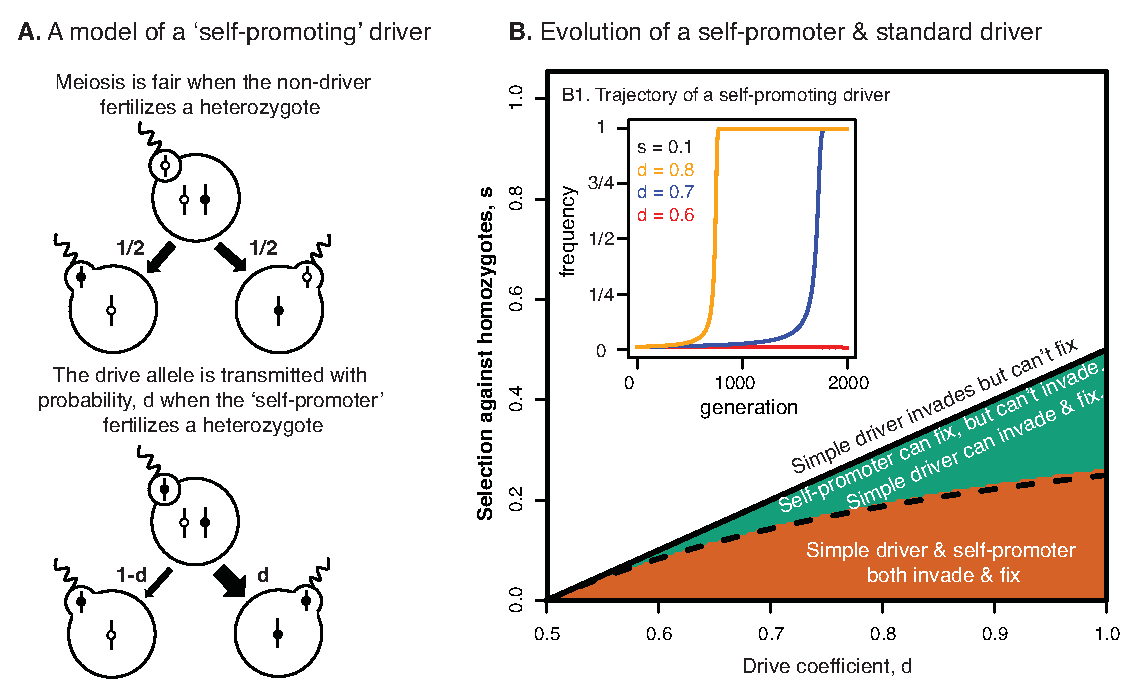
\includegraphics[width = 1 \textwidth]{../Figures/selfprom.eps} \end{center}
\caption{{\bf{A.}} A visual depiction of our model of `self-promoting' driver. 
	Transmission probabilities for alleles through female
 	 meiosis depend on sperm genotype. 
	 The non-driving $A$-allele, and self-promoting $B$-allele
	 are represented by unfilled and filled circles, respectively. 
	 {\bf{B.}} Evolution of a self-promoter and standard driver. 
	 	Assuming that the fitnesses of drive homozygotes and 
		heterozygotes are $1-s$ and $1$, respectively. 
	 	\emph{Main figure:} Boundary conditions for the invasion 
		and fixation of self-promoting and standard meiotic drivers, 
		with drive coefficient, $d$. Colored regions depict exact results, 
		while lines  represent analytical approximations. 
	 \emph{B1:}  Trajectories of sperm-dependent female drive
		 %alleles that can invade the population, 
		 each allele has $s =0.1$ against the
		 homozygotes.  The drive coefficient is denoted by color. 
 }   
\label{Eggsperm}
\end{figure}

\clearpage
\newpage

\begin{figure}
\begin{center}
%	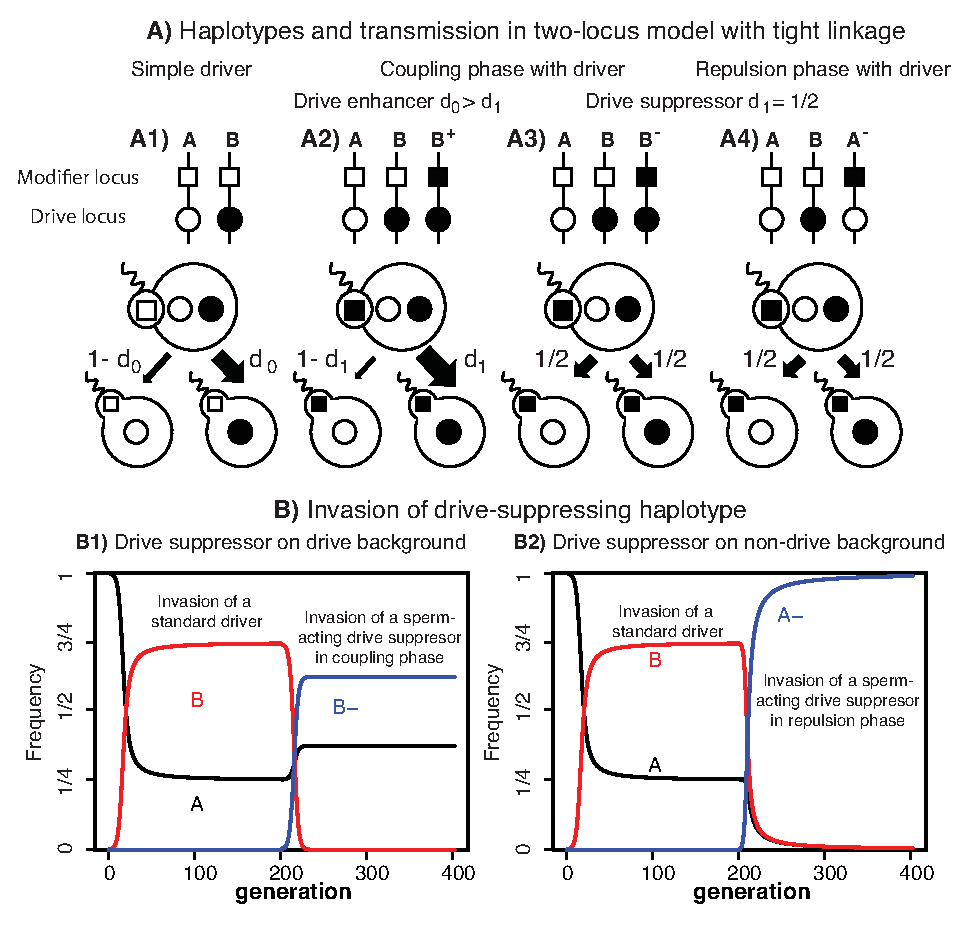
\includegraphics[width = 0.7 \textwidth]{../Figures/twolocus.eps} 
          \end{center}
\caption{Models of a sperm-acting drive modifier tightly linked to a meiotic driver. 
{\bf (A) } 
Sperm carrying the derived allele at the modifier locus (filled squares) alters transmission  
	at the driving allele (filled circles) during female meiosis.
        Alleles at these two tightly linked loci form three haplotypes (top of A). 	
	{\bf{A1)}} In the standard model of drive there is no
        variation at the modifier, 
	and the driver is transmitted to the egg with probability $d_0$. 
	{\bf{A2)}} The modifier allele increases the transmission of the drive allele ($d_1 > d_0$), and due to their shared genetic background, also increases its drive. 
	{\bf{A3 \& A4)}} The sperm-acting modifier acts to decrease
        drive  ($d_1=1/2$ in A3 \& A4, or more generally, $d_1 < d_0$) and arises on the same or opposite
        background from the driver (A3 \& A4 respectively). 
{\bf{(B)}} Invasion of a sperm-acting drive suppressor linked to a driver. 
	After the driver ($B$ haplotype) reaches drive selection equilibrium, we introduce a sperm acting drive modifier. 
	We assume full drive ($D_0 =1$), a recessive lethal fitness cost to drive ($h_s=0$, $s=1$) and that the sperm-acting modifier results in a fair meiosis. 
{\bf {B1)}} The $B^-$ allele replaces the ancestral drive haplotype, but segregates at a lower equilibrium frequency.
{\bf {B2)}} The $A^-$ allele replaces the ancestral non-driving haplotype, and in this case, removes the driver from the population. }
 \label{Eggsperm_3_allele_cartoon}
\end{figure}

\clearpage
\newpage
  \setcounter{figure}{0}\global\def\thefigure{S\arabic{figure}}

\section*{Supplementary Material}

{\bf{File S1:}} Transmission rules. We detail the frequency of offspring genotypes produced by each possible mating for Models 1-6 in the tabs of this Excel spreadsheet. 
\\ \\
{\bf{Files S2A \& S2B:}} A Mathematica file (FileS2A) and a PDF of this file (File S2B) in which we derive analytical results for models 1-6 and $6^\prime$. 
\\ \\
{\bf{File S3:}} Exact approach. The R Script used for exact recursions for all models, including cases with inbreeding.
\\ \\
{\bf{File S4:}} Variation in critical time-points during female meiosis across taxa (adapted from \citet{Masui_book}).
\\ \\
{\bf{File S5:}} An R object containing the phylogeny and raw data used to generate Figure \ref{Meiotic_fig}.
\\ \\
{\bf{File S6:}} The R Script used to generate Figure \ref{Meiotic_fig}. This requires that File S5 is loaded into the R environment.
\clearpage

\newpage
\subsection*{Supplementary Figure Legends}
\clearpage


\begin{figure}
%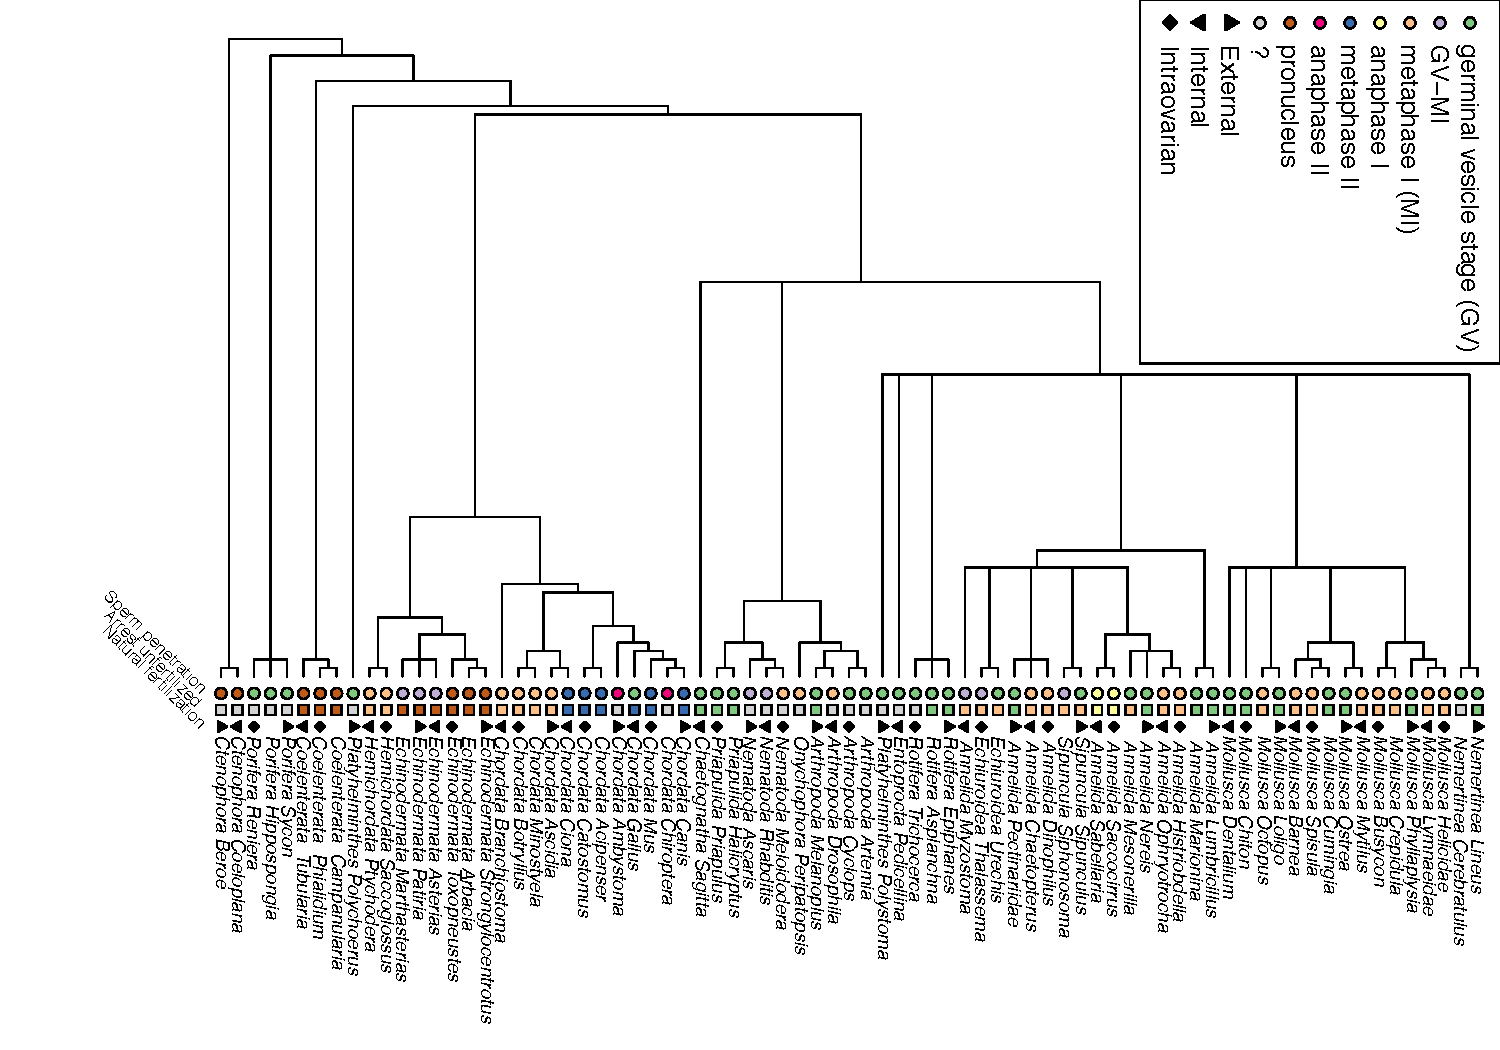
\includegraphics[width = \textwidth]{supp/meiotic_phylogeny.pdf}
\caption{The phylogenetic distribution of the female meiotic
  arrest. The first two columns of symbols gives the stage of the ooycte when
  the sperm penetrates and the stage at which it arrests if
  unfertilized. The third column of symbols shows the site for natural fertilization. 
  These columns of phenotypic data were extracted from Table
  1 of \citet{Masui_book}. The tree was extracted from the Open Tree of
Life project. The raw data table, the phylogeny/supporting R objects, and the script to do this is are included in
the supplement (Files S4-S6). }  
\label{Meiotic_fig}
\end{figure}


\begin{figure}
%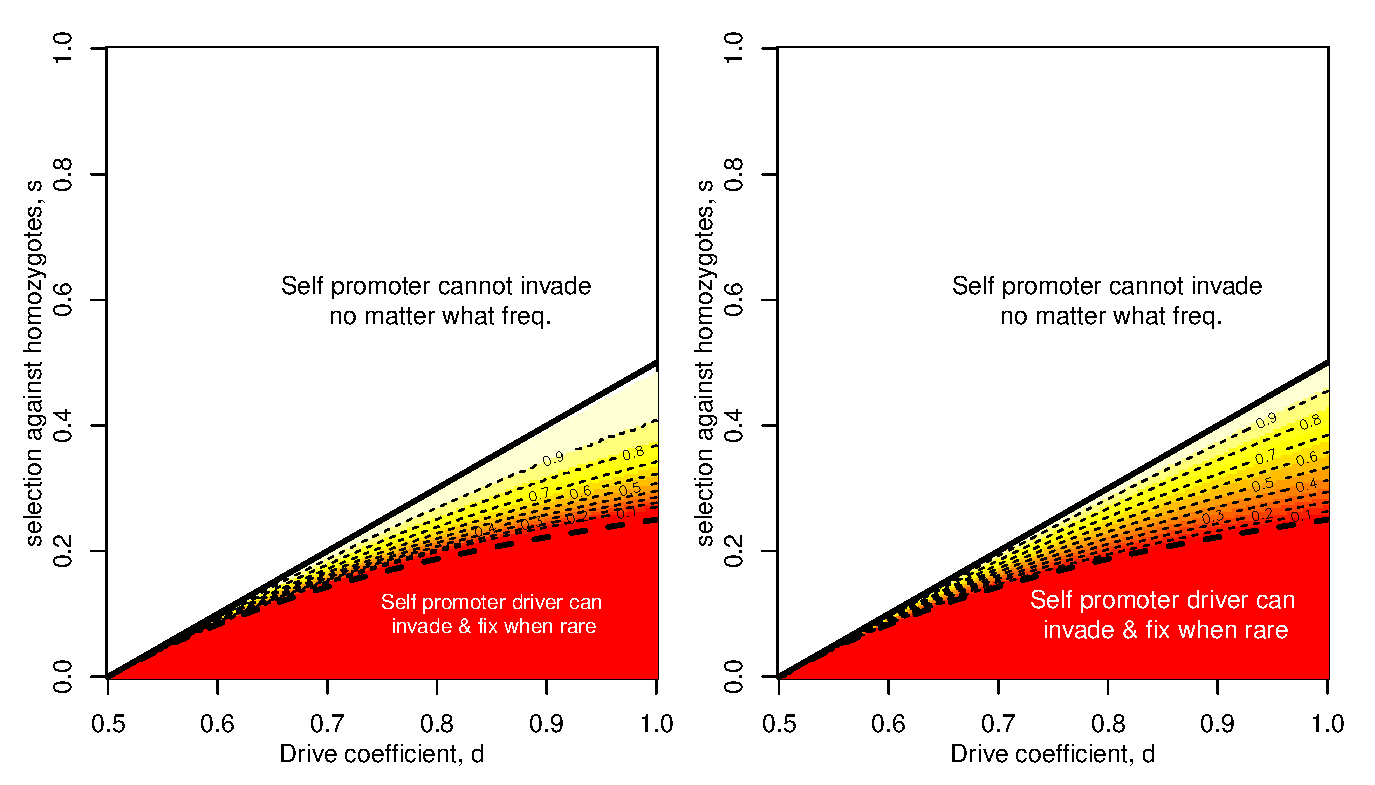
\includegraphics[width = \textwidth]{../../Scripts/homozyg_bistability.eps}
\caption{Invasion analysis for a self-promoting female meiotic drive allele with
  recessive costs (selection coefficient $s$), showing the region of
  bistability. The colors, and the thin dashed contours, indicate the
  frequency the allele must reach, $f^*$ in order to invade the population (note
  that these alleles reach fixation conditional on invading). In the
  white area, the allele cannot invade, in the solid red
  area the allele can invade and fix when rare. In the left panel we
  show the results obtained by a grid search using the recursion, on
  the right we show the approximation obtained assuming that HWE
  holds. }  
\label{Bistab_homozyg_cost_fig}
\end{figure}

\begin{figure}
%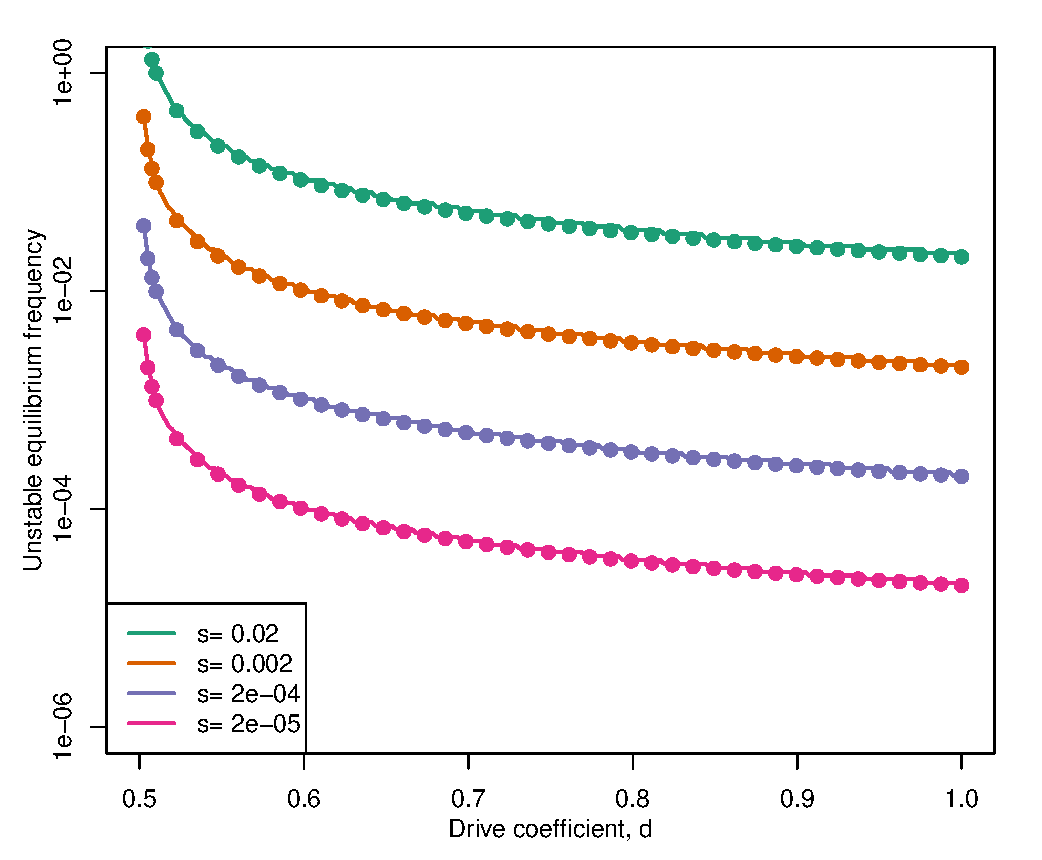
\includegraphics[width = 0.8 \textwidth]{../Figures/bistable_x_vs_d_additive_s.eps} 
\caption{The unstable equilibrium frequency for a self-promoting
  female meiotic drive allele with an additive cost ($s_h=s/2$) as a
  function of the drive parameter. The solid line shows results
  obtained using the recursion, the dots our approximation given by Equation \eqref{thresh2}}  \label{bistable_additive}
\end{figure}

\begin{figure}
%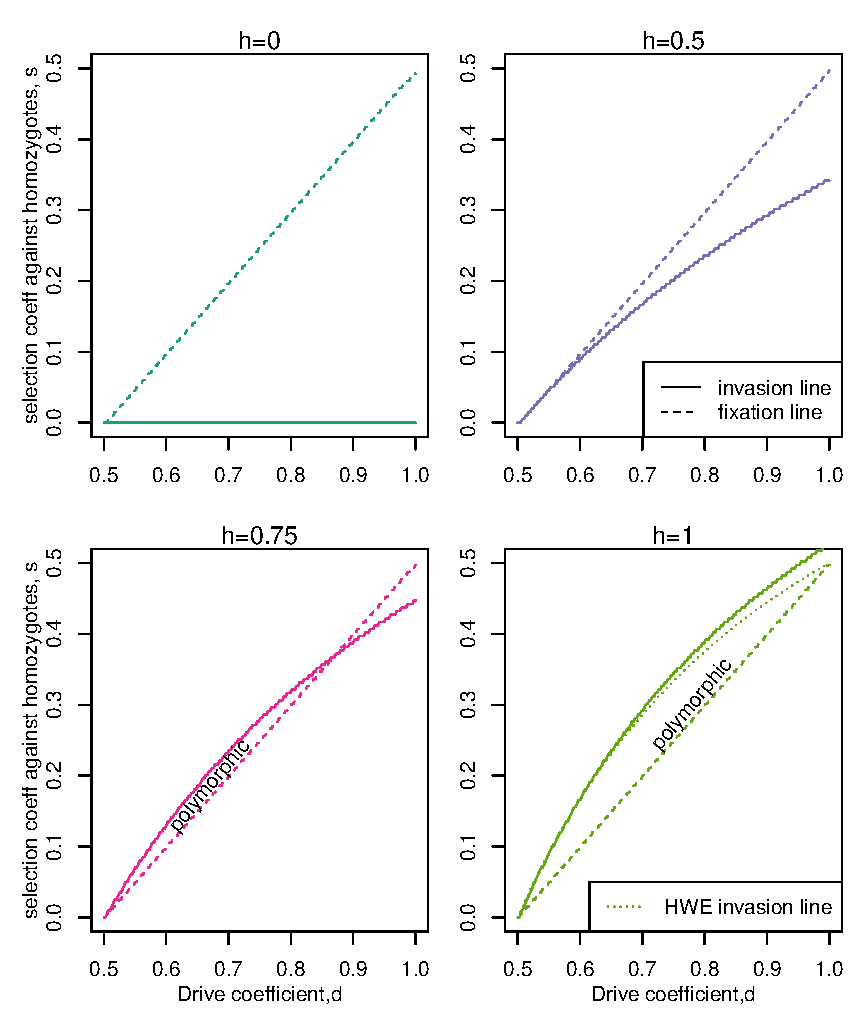
\includegraphics[width = 0.7 \textwidth]{../../Scripts/effect_of_dominance_on_invasion_space_four_graph.eps} 
\caption{Exact results of invasion analysis of an allele whose effect
 on female meiosis is mediated by the genotype of the fertilizing
 male.  
 A heterozygous female transmits the $B$ allele 
  with probabilities  $\frac{1}{2}$,  $d_{het}=\frac{1}{2} + h(d_{hom}-\frac{1}{2}) $ or $d_{hom}$, 
 if she mated with a n $AA$, $AB$, or $BB$ male,  respectively.  
 The allele suffers a recessive fitness cost $s$.  
 The four panels correspond to different dominance relationships.
In the parameter space below the invasion (solid) line the self-promoter
 driver can invade. In the parameter space below the fixation (long
 dash) line the self-promoter can fix. In the last
 two panels the invasion line is above the fixation line and so the
 allele can be maintained as a polymorphism in that thin slice of
 parameter space between the two lines. 
 In the final panel we show the
  fixation line (small dashes) as predicted by our HWE approximation
  ($(d_{het}-1/2)/d_{het}$) see the appendix for more details.
}  \label{Effect_of_dominance}
\end{figure}

\begin{figure}
%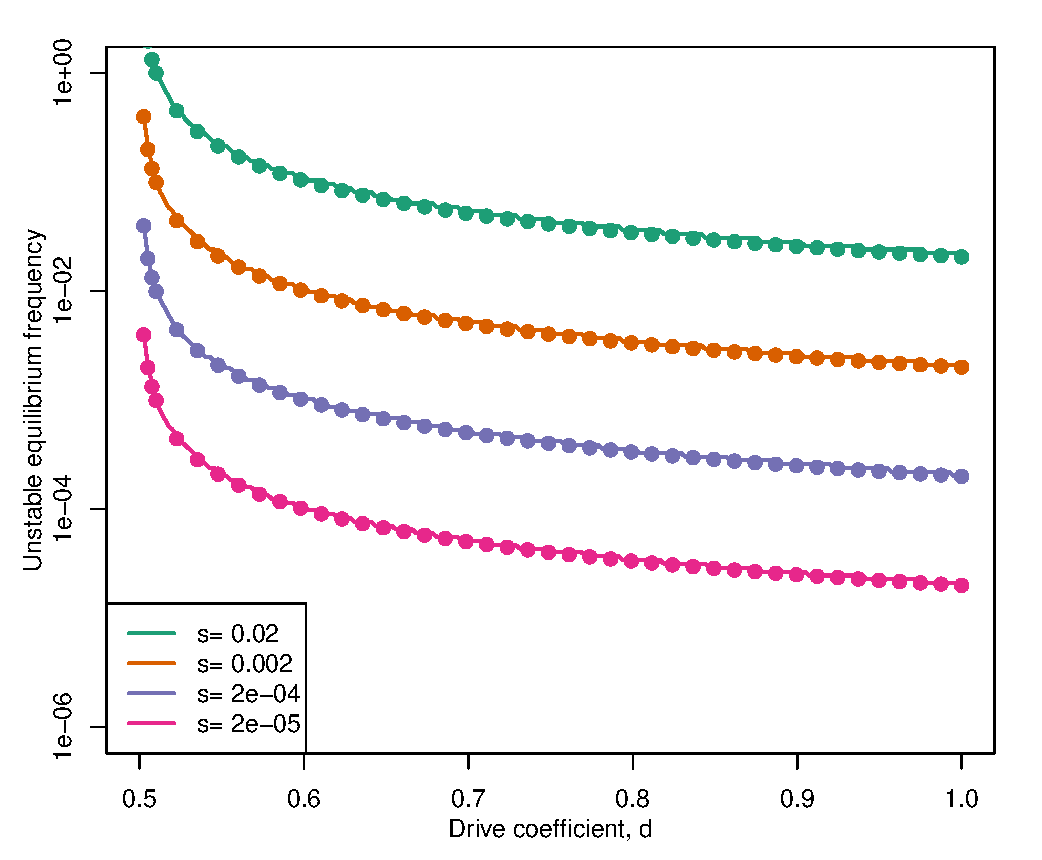
\includegraphics[width = 0.8 \textwidth]{../Figures/bistable_x_vs_d_additive_s.eps} 
\caption{Evolution of a self-promoter and standard driver with variable levels of inbreeding (modifying the selfing rate from 0 to 0.9, in 0.1 increments). 
	 	Assuming that the fitnesses of drive homozygotes and 
		heterozygotes are $1-s$ and $1$, respectively. 
	 	Boundary conditions for the invasion (solid lines) 
		and fixation (dotted lines) of self-promoting (red) and standard (black) meiotic drivers, 
		with drive coefficient, $d$. 
		We derived these conditions from the simulation in File S3.}
		\label{self}
\end{figure}


\end{document}




